\documentclass{CUP-JNL-DTM}%


%%%% Packages
\usepackage{graphicx}
\usepackage{multicol,multirow}
\usepackage{amsmath,amssymb,amsfonts}
\usepackage{mathrsfs}
\usepackage{amsthm}
\usepackage{rotating}
\usepackage{appendix}
% For JDM please remove the natbib package:
% And use biblatex-apa with a .bib file to format your references according to the APA7 style.
\usepackage[style=numeric, backend=biber]{biblatex}
\addbibresource{refs.bib} % or whatever your .bib file is called
\usepackage{ifpdf}
\usepackage[T1]{fontenc}
\usepackage{newtxtext}
\usepackage{newtxmath}
\usepackage{textcomp}
\usepackage{xcolor}
\usepackage{lipsum}
\usepackage{float}
\usepackage{subcaption}
\usepackage[colorlinks,allcolors=blue]{hyperref}


\newtheorem{theorem}{Theorem}[section]
\newtheorem{lemma}[theorem]{Lemma}
\theoremstyle{definition}
\newtheorem{remark}[theorem]{Remark}
\newtheorem{example}[theorem]{Example}
\numberwithin{equation}{section}


\jname{Universidad San Francisco de Quito}
\articletype{}
\artid{}
\jyear{2025}
\jvol{}
\jissue{}
\raggedbottom


\begin{document}

\begin{Frontmatter}

\title[Article Title]{High Energy Physics Final Project}

% There is no need to include ORCID IDs in your .pdf; this information is captured by the submission portal when a manuscript is submitted. 
\author[1]{Jos\'e David Ochoa Flores}

\authormark{Author Name1 \textit{et al}.}

\address[1]{\orgdiv{Maestr\'ia de F\'isica}, \orgname{Universidad San Francisco de Quito}, \orgaddress{\city{Quito}, \country{Ecuador}}}


\authormark{Jos\'e Ochoa}

\keywords{Simulation chain, Drell-Yan, Beyond Standard Model, Higgs, FeynRules}

\abstract{The following project aims to recreate a full simulation chain of a Drell-Yan (DY) process in a Beyond the Standard Model (BSM) model and compare the results with the usual DY process. For this, we use FeynRules, MadGraph, Pythia, CMSSW and Python with several packages such us uproot. The final resuls show no difference whatsoever between the two models, this is most likely a result of the poor number of events that we are able to generate locally. All the code used in this project can be found in my personal github page \cite{jose8afHEPProject}}

\end{Frontmatter}

% Some math journals (FLO) require a table of contents. Comment out this line if no ToC is needed.
%\localtableofcontents

\section{Introduction}
Simulations in high-energy physics play a crucial role in understanding the dynamics of both Standard Model (SM) and Beyond the Standard Model (BSM) processes. A variety of computational tools have been developed to support this effort, enabling the implementation of theoretical models and the generation of realistic collider events.

Among the most widely used tools are:
\begin{itemize}
    \item \textit{FeynRules}~\cite{Alloul:2013bka}, which allows for the implementation of new physics models by deriving Feynman rules from a Lagrangian;
    \item \textit{MadGraph5\_aMC@NLO}~\cite{Alwall:2014hca}, which simulates parton-level events for both SM and BSM processes;
    \item \textit{Pythia}~\cite{Sjostrand:2014zea}, used for parton showering and hadronization;
    \item and the \textit{CMS Software Framework (CMSSW)}, which performs full detector simulation.
\end{itemize}

This project focuses on the Hidden Abelian Higgs Model (HAHM), implemented via FeynRules and exported to MadGraph for event generation. The HAHM is a well-motivated BSM scenario where a hidden $U(1)_X$ gauge symmetry introduces a new massive gauge boson and scalar state, with the potential for exotic Higgs decays~\cite{Curtin:2013fra,Curtin:2014cca}.




\section{Hidden Abelian Higgs Model (HAHM)}

The Hidden Abelian Higgs Model (HAHM) extends the Standard Model (SM) by introducing an additional $U(1)_X$ gauge symmetry with gauge boson $\hat{X}_\mu$ that kinetically mixes with the SM hypercharge boson $\hat{B}_\mu$. The corresponding kinetic Lagrangian is:
\begin{equation}
\mathcal{L}_X = -\frac{1}{4} \hat{X}_{\mu\nu} \hat{X}^{\mu\nu} + \frac{\chi}{2} \hat{X}_{\mu\nu} \hat{B}^{\mu\nu},
\end{equation}
where $\chi$ is the kinetic mixing parameter, assumed to be small.

To break $U(1)_X$ spontaneously, a complex scalar SM-singlet field $\Phi_H$ charged under $U(1)_X$ is introduced. The extended scalar sector Lagrangian is:
\begin{equation}
\begin{aligned}
\mathcal{L}_\Phi &= |D_\mu \Phi_{SM}|^2 + |D_\mu \Phi_H|^2 + \mu^2_{\Phi_H} |\Phi_H|^2 + \mu^2_{\Phi_{SM}} |\Phi_{SM}|^2 \\
&\quad - \lambda |\Phi_{SM}|^4 - \rho |\Phi_H|^4 - \kappa |\Phi_{SM}|^2 |\Phi_H|^2,
\end{aligned}
\end{equation}
where $\Phi_{SM}$ is the SM Higgs doublet, and $\kappa$ controls Higgs-portal mixing.

After spontaneous symmetry breaking, the vacuum expectation values are
\[
\langle \Phi_H \rangle = \frac{\xi}{\sqrt{2}}, \quad \langle \Phi_{SM} \rangle = \left(0, \frac{v}{\sqrt{2}}\right).
\]

\subsection{Mass Eigenstates and Mixing}

\textbf{Gauge Sector:} Kinetic mixing leads to mass mixing between the SM $Z$ boson and the new $U(1)_X$ boson. After diagonalization, the physical states are $Z$ and $Z_D$, with a mixing angle $\theta_a$ defined by:
\begin{equation}
\tan(2\theta_a) = \frac{-2 s_W \eta}{1 - s_W^2 \eta^2 - \Delta_Z},
\end{equation}
where $\eta = \chi / \sqrt{1 - \chi^2}$ and $\Delta_Z = M_X^2 / M_Z^2$.

\textbf{Higgs Sector:} The neutral scalars mix via the $\kappa$ interaction. The physical eigenstates $h$ (SM-like) and $h_s$ (singlet-like) are defined via:
\begin{equation}
\tan(2\theta_h) = \frac{\kappa v \xi}{\rho \xi^2 - \lambda v^2}.
\end{equation}

\subsection{New Parameters and Couplings}

\begin{itemize}
    \item $\chi$ (kinetic mixing) $\rightarrow$ $\epsilon = \chi / \cos \theta_W$
    \item $\kappa$ (Higgs portal coupling)
    \item $M_{Z_D}, M_{h_s}$ (new mass eigenvalues)
\end{itemize}

The couplings of the new gauge boson $Z_D$ to SM fermions, and of the Higgses to gauge bosons and fermions, are modified as functions of $\theta_{a}$ and $\theta_{h}$. For example, Higgs decays to $Z_D Z_D$ or $Z_D \rightarrow l+ l-$ are allowed if kinematically accessible. This is important as we seek to study the Drell-Yan process, which is mediated by the exchange of a $Z$ boson.



\section{Simulation Chain}

The simulation chain consists of several steps, each performed using specific software tools. The process begins with the implementation of the HAHM model in FeynRules, here we calculate the Feynman Rules and export the results in a directory with a UFO format, after this the generation of events is done using MadGraph, in our case the process generated was $p p \rightarrow l^+ l^-$. It was also possible to include at this step of the simulation the pythia hadronization process. It is worth noting that MadGraph also allows to include the detector simulation, but the processs seems to be more intricated. Finally we use CMSSW for full detector simulation. This includes a series of steps using $cmsDriver$, a tool used to generate the configuration files in a easier way. The final step involves analyzing the results using Python and uproot. A general overview of the simulation chain is shown in Figure \ref{fig:chain}.

\begin{figure}[H]
  \centering
  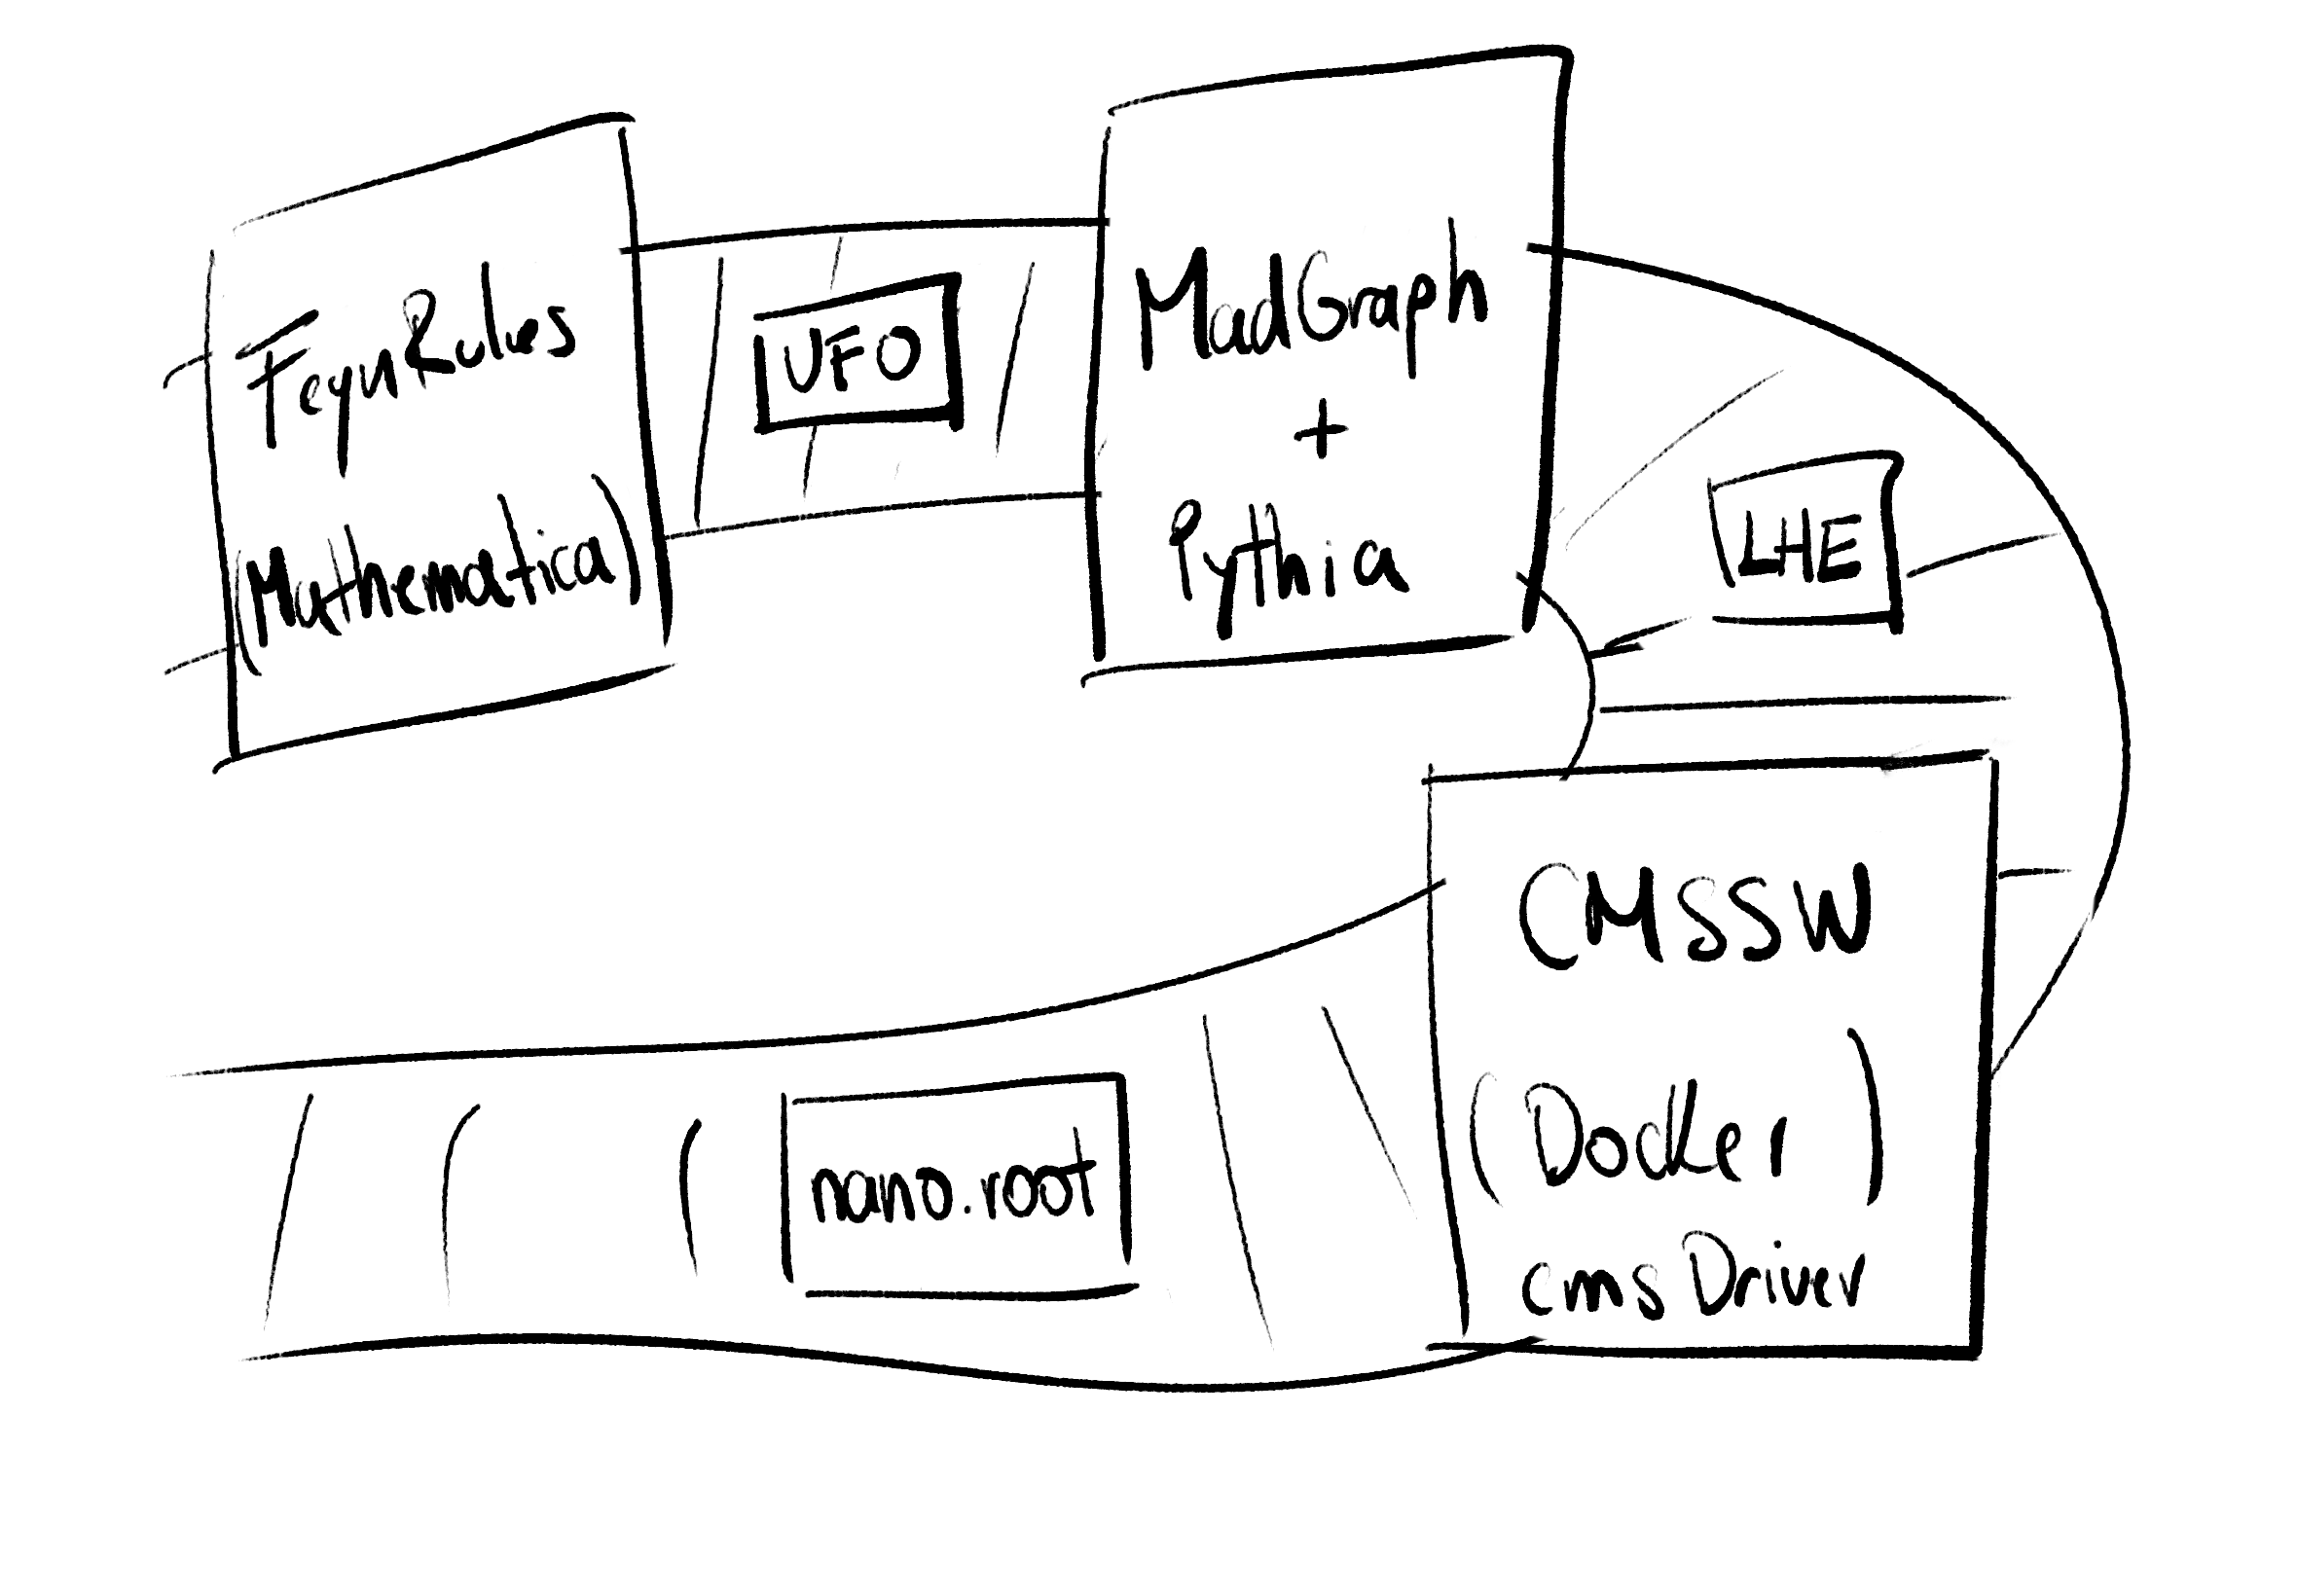
\includegraphics[width=0.85\linewidth]{img/chain.png}
  \caption{The simulation chain machine}
  \label{fig:chain}
\end{figure}

Before going into the result section it may be interesting to show the different type of diagrams that we can obtain from the SM DY and BSM DY processes. The Feynman diagrams for the SM DY process are shown in Figure \ref{fig:sm_dy}, while the BSM DY process is shown in Figure \ref{fig:bsm_dy}. The main difference between the two models is the number of possible diagrams for a $p p \rightarrow l^+ l^-$ process, acounting for up to 84 diagrams in the BSM model. This makes sense as there is now a new gauge boson $Z_D$ and a new $h_s$ Higgs in the BSM model, which can couple to leptons. There is also the extra posibility of the $h_s$ coupling to gluons as seen in the diagrams below which also increases the possible diagrams.

\begin{figure}[H]
  \begin{subfigure}{.5\textwidth}
    \centering
    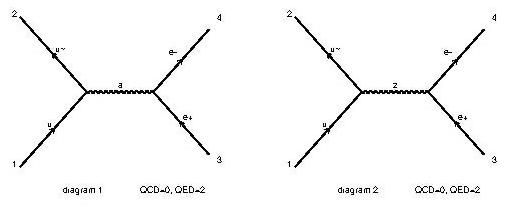
\includegraphics[width=1\linewidth]{img/dy_sm_diagrams.jpg}
    \label{fig:sm_dy1}
  \end{subfigure}%
  \begin{subfigure}{.5\textwidth}
    \centering
    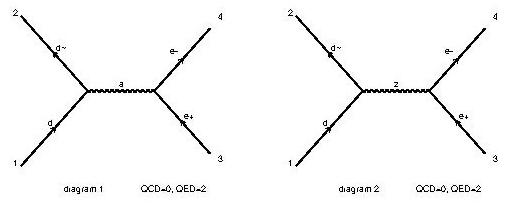
\includegraphics[width=1\linewidth]{img/dy2_sm_diagrams.jpg}
    \label{fig:sm_dy2}
  \end{subfigure}
  \caption{SM DY feynman diagrams}
  \label{fig:sm_dy}
\end{figure}



\begin{figure}[H]
  \begin{subfigure}{.5\textwidth}
    \centering
    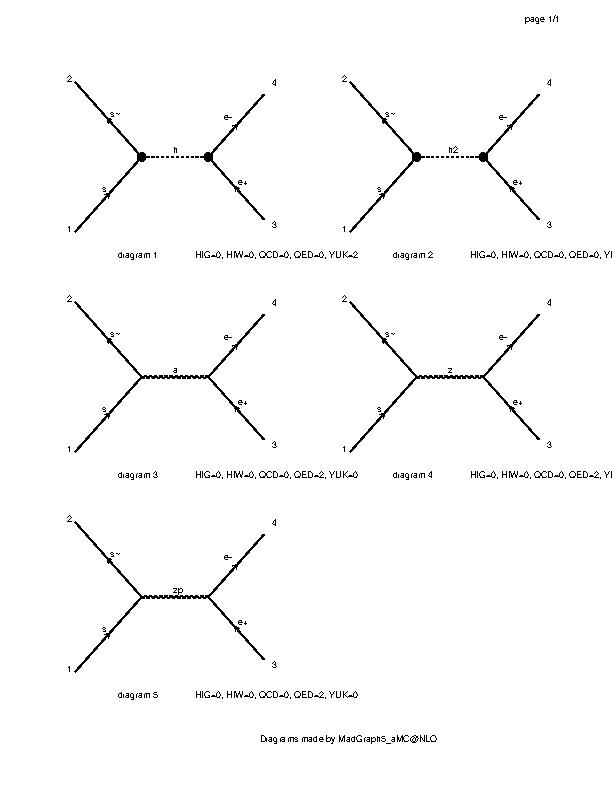
\includegraphics[width=1\linewidth]{img/dy_bsm_diag.jpg}
    \label{fig:bsm_dy1}
  \end{subfigure}%
  \begin{subfigure}{.5\textwidth}
    \centering
    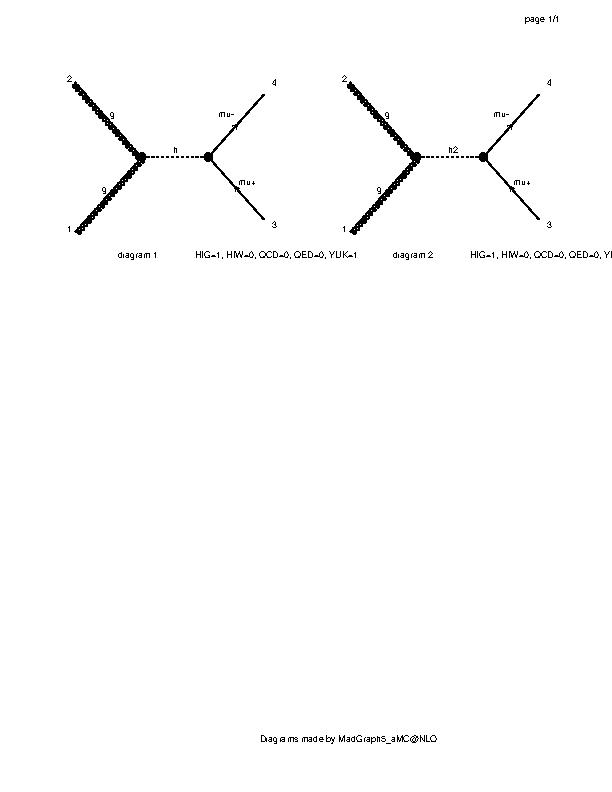
\includegraphics[width=1\linewidth]{img/bsm_dy_diag2.jpg}
    \label{fig:bsm_dy2}
  \end{subfigure}
  \caption{BSM DY feynman diagrams}
  \label{fig:bsm_dy}
\end{figure}



\section{Results}
All the code used in this project can be found in my personal github page \cite{jose8afHEPProject}. This includes the UFO directory, the LHE files, the cmsDriver steps and the python scripts used to analyze the results. 
To analyze the results a several amount of histograms were made. This included the invariant mass of the dilepton system, the transverse momentum of the MET and PuppiMET, and the phi angle of the MET and PuppiMET. The results were compared between the SM DY and BSM DY processes. The results are shown in the Figures below. 


\begin{figure}[H]
    \begin{subfigure}{.5\textwidth}
      \centering
      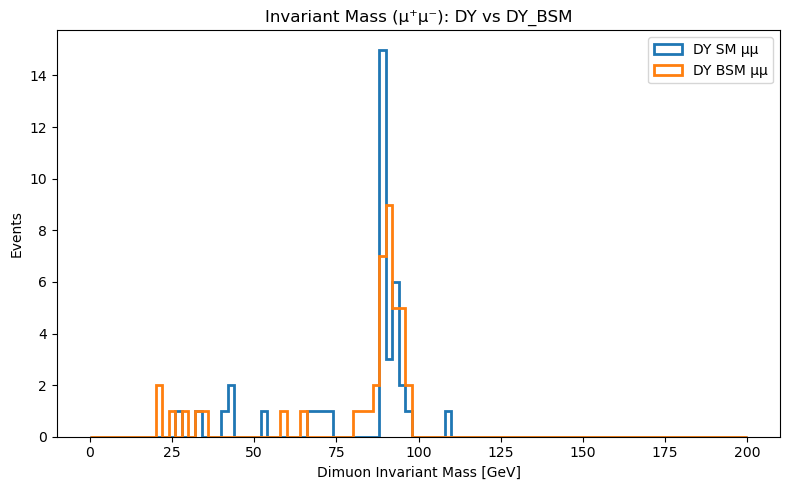
\includegraphics[width=.85\linewidth]{img/mumu_comp.png}
      \caption{Dimuon invariant mass}
      \label{fig:mumu}
    \end{subfigure}%
    \begin{subfigure}{.5\textwidth}
      \centering
      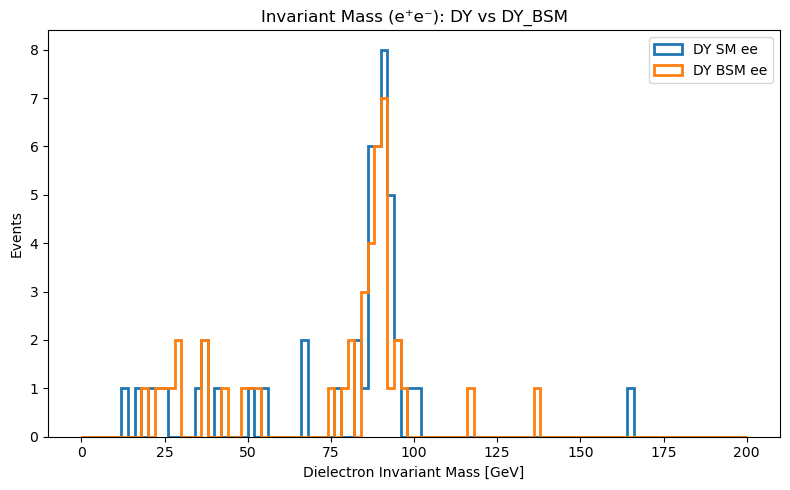
\includegraphics[width=.85\linewidth]{img/ee_comp.png}
      \caption{Dielectron invariant mass}
      \label{fig:ee}
    \end{subfigure}
    \caption{Dilepton invariant mass comparison for SM DY and BSM DY} 
    \label{fig:imass}
\end{figure}



\begin{figure}[H]
    \begin{subfigure}{.5\textwidth}
      \centering
      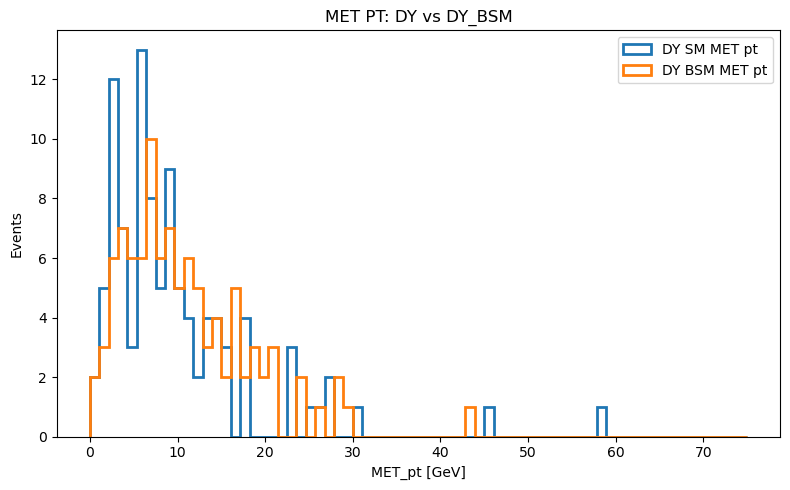
\includegraphics[width=.85\linewidth]{img/met_pt.png}
      \caption{MET pt}
      \label{fig:sm_metpt}
    \end{subfigure}%
    \begin{subfigure}{.5\textwidth}
      \centering
      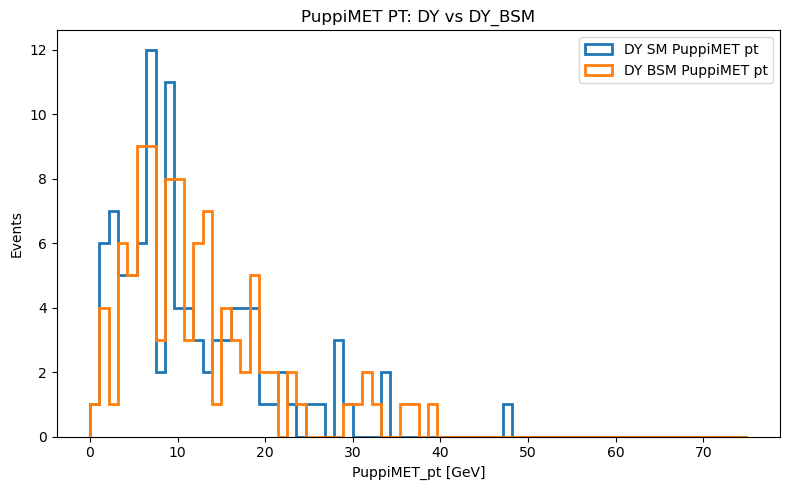
\includegraphics[width=.85\linewidth]{img/pmet_pt.png}
      \caption{PuppiMET pt}
      \label{fig:sm_pmetpt}
    \end{subfigure}
    \caption{MET pt and PuppiMET pt comparison for SM DY and BSM DY}
    \label{fig:metpt}
\end{figure}

\begin{figure}[H]
    \begin{subfigure}{.5\textwidth}
      \centering
      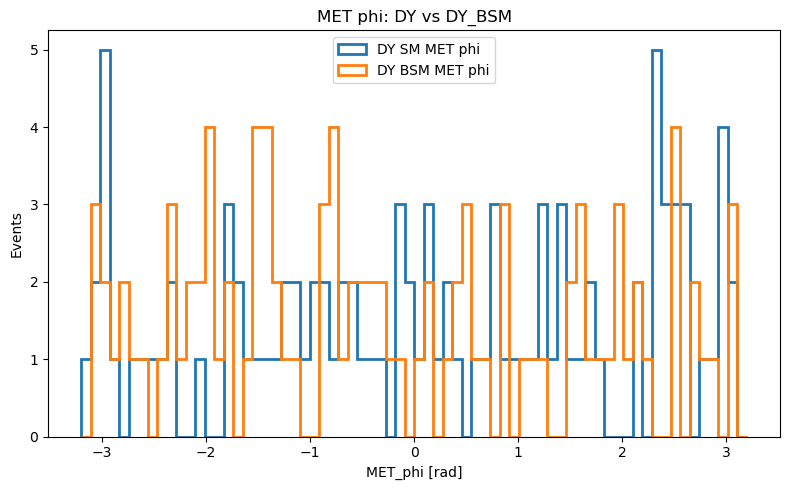
\includegraphics[width=.85\linewidth]{img/met_phi.png}
      \caption{MET phi}
      \label{fig:sm_metphi}
    \end{subfigure}%
    \begin{subfigure}{.5\textwidth}
      \centering
      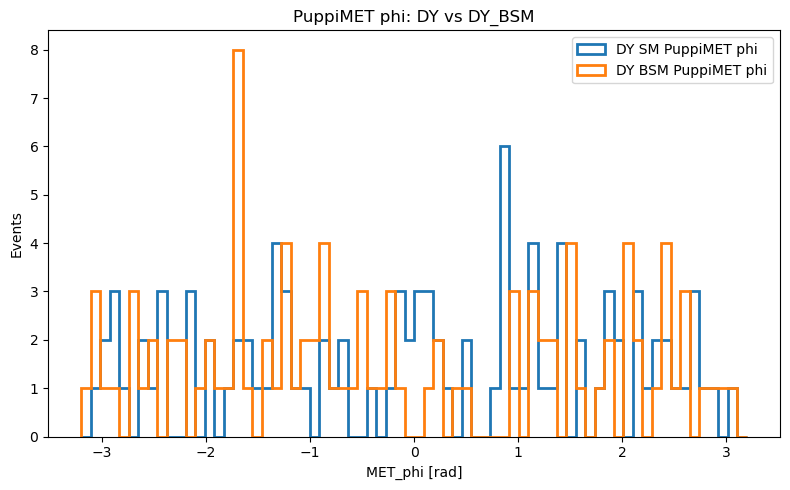
\includegraphics[width=.85\linewidth]{img/pmet_phi.png}
      \caption{PuppiMET phi}
      \label{fig:sm_pmetphi}
    \end{subfigure}
    \caption{MET phi and PuppiMET phi comparison for SM DY and BSM DY}
    \label{fig:metphi}
\end{figure}

\section{Conclusion}
A slight broadening in the BSM MET and BSM PUPPI MET $p_T$ distributions is visible in Figure~\ref{fig:metpt} when compared to the SM Drell-Yan. A small displacement between the BSM and SM distributions is also noticeable in the same figure. However, these differences are minimal, highlighting that the limited number of generated events is a significant constraint in this study.

Aside from the small differences mentioned, the results show essentially no meaningful deviation between the two models. A more extensive simulation with a larger event sample is required to draw robust conclusions. A possible next step would be to compare the $h_s$ decay with the SM Higgs decay, where a larger discrepancy may emerge.

\begin{Backmatter}

\printbibliography


\end{Backmatter}


\end{document}
